One of the most important documents that teams will need to create is the CONOPS, which requires most of its data from this Behavior section of the Reference Architecture. Figure \ref{fig:Behavior Organization} shows the top level organization of the Behavior package with the key diagrams that ultimately fill out the CONOPS document. 

\begin{figure}[H]
    \centering
    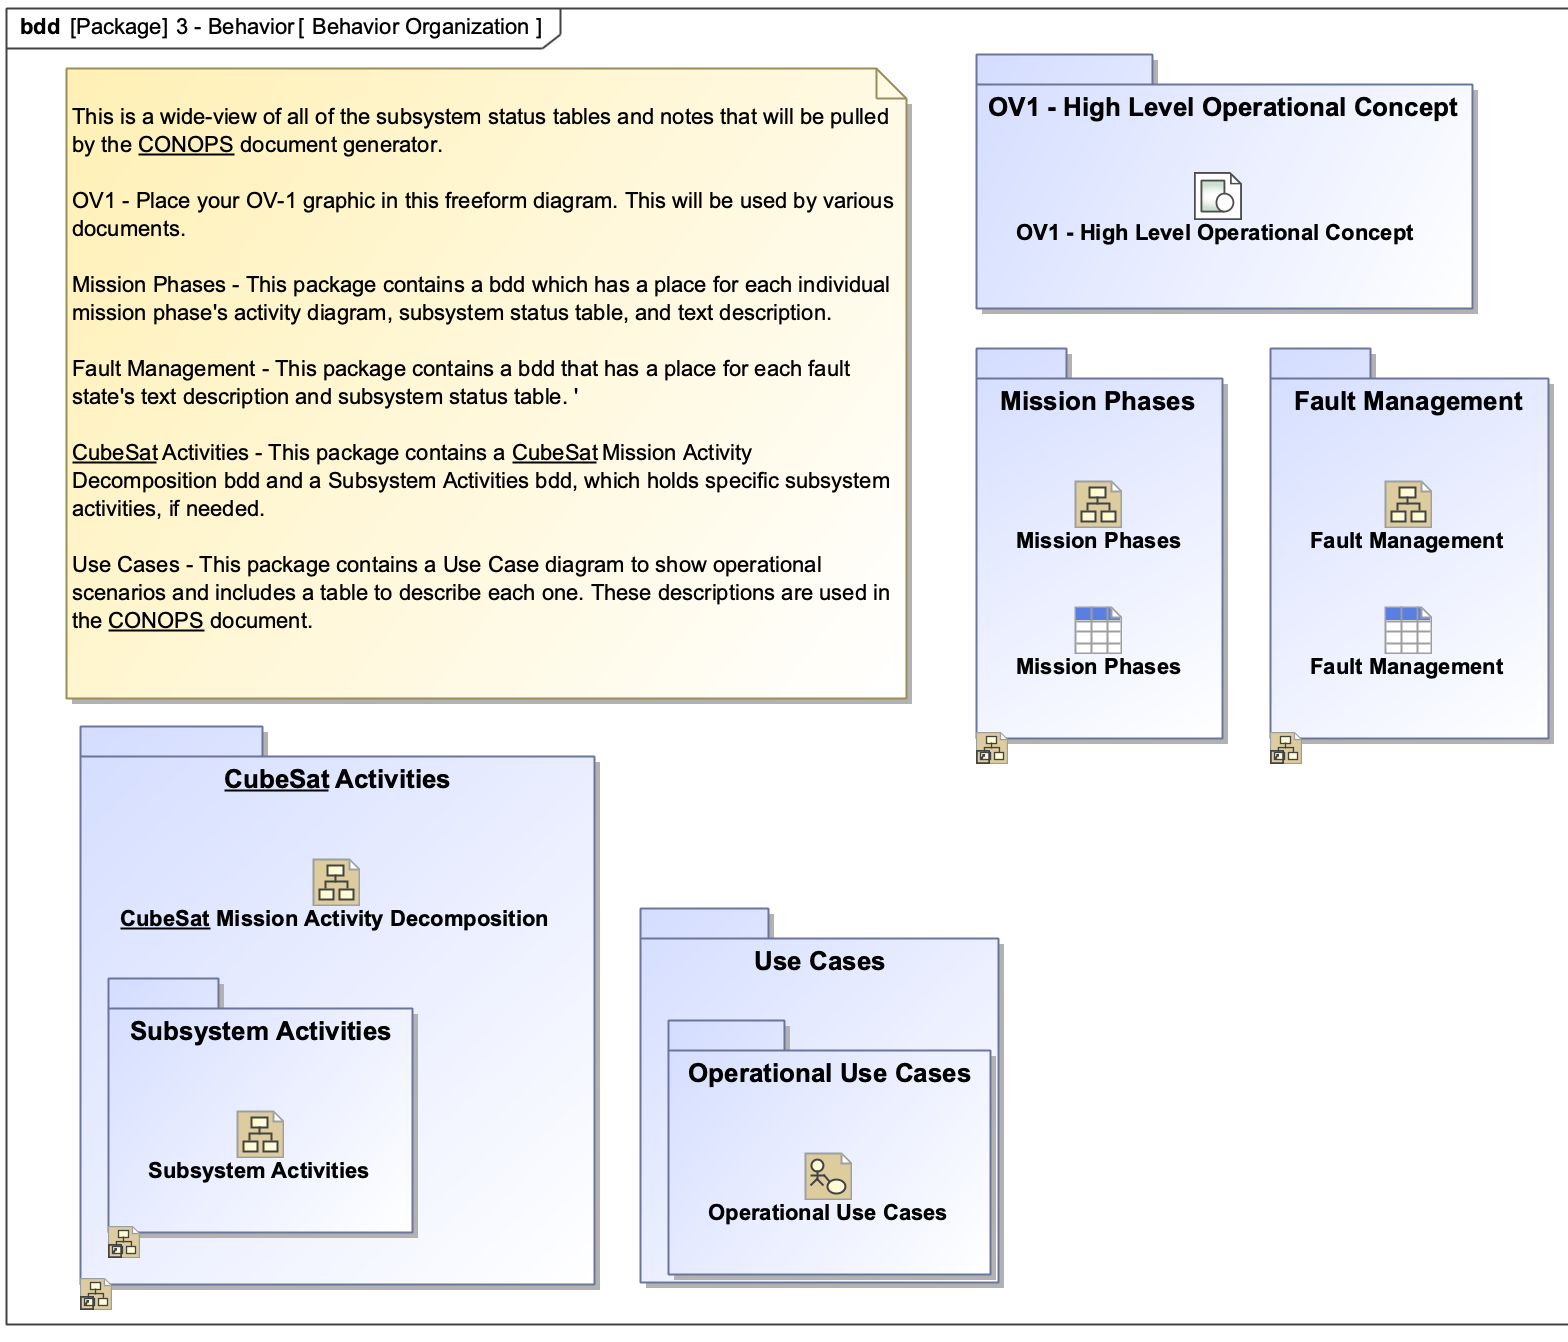
\includegraphics[width=\textwidth]{Thesis/Analysis_and_Results/Analysis and Results Figures/Behavior Organization.png}
    \caption{Behavior Organization}
    \label{fig:Behavior Organization}
\end{figure}

The note in Figure \ref{fig:Behavior Organization} describes what teams should use each included package for, and each package is hyperlinked to more detailed diagrams to fill out.  

A template OV-1 has been included in a free form diagram, and teams will replace this template image with their own so that documents can include the image automatically. The OV-1 is a “High Level Operational Concept Graphic,” usually a preferred view of a mission from Senior Leaders.  The Department of Defense Architecture Framework describes it as “a mission, class of mission, or scenario. It shows the main operational concepts and interesting or unique aspects of operations. It describes the interactions between the subject architecture and its environment, and between the architecture and external systems. The OV-1 is the pictorial representation of the written content of the AV-1 Overview and Summary Information. Graphics alone are not sufficient for capturing the necessary architectural data. The OV-1 provides a graphical depiction of what the architecture is about and an idea of the players and operations involved. An OV-1 can be used to orient and focus detailed discussions. Its main use is to aid human communication, and it is intended for presentation to high-level decision-makers. \citep{DoDAF}” 

The Mission Phases package (Figure \ref{fig:Mission Phases}) contains a block definition diagram which has a place for each individual mission phase's activity diagram, subsystem status table, and text description. During each mission phase, the CubeSat’s various subsystems will be in unique configurations, and this package includes an easy way to capture those. To capture these different configurations, tables have been created for teams to determine the various states for each subsystem for each phase. In addition to the subsystem configuration tables, teams should write textual descriptions of the applicable mission phase in the “Mission Phases” table (Figure \ref{fig:Mission Phase Descriptions}) and create activity diagrams to show what happens in each phase. All of these will be used in the CONOPS document. 

\begin{figure}[H]
    \centering
    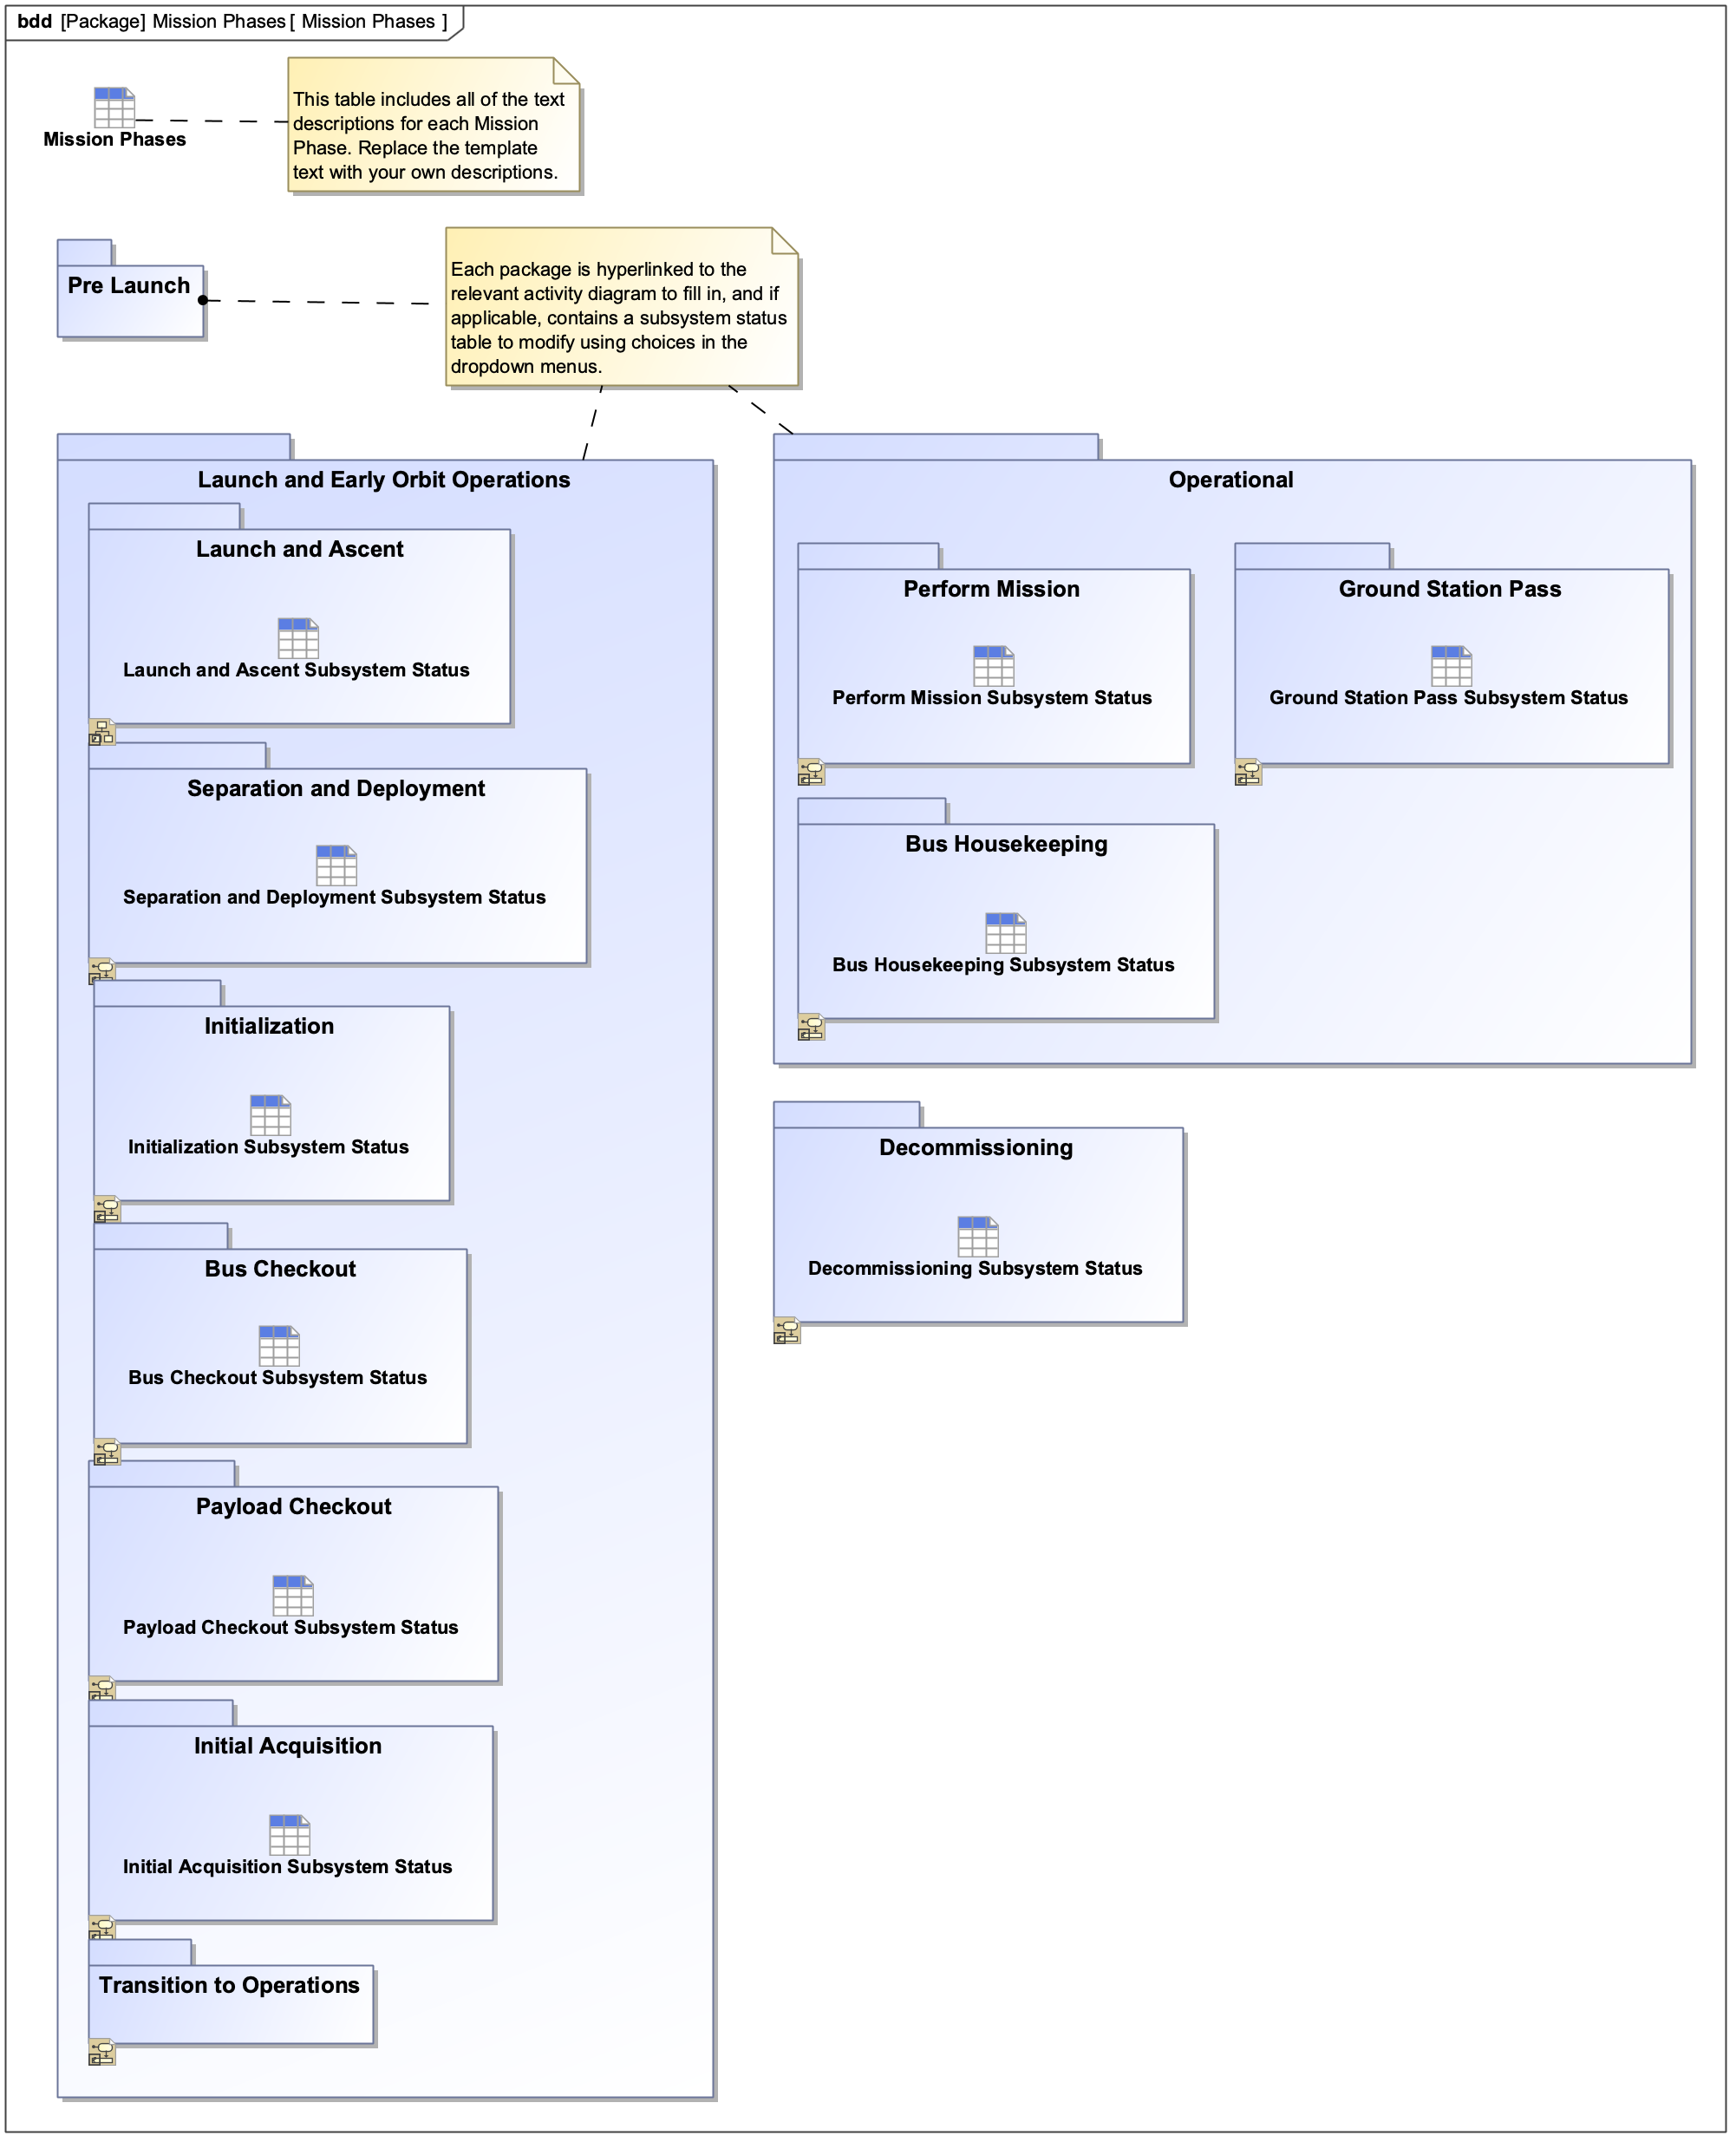
\includegraphics[width=\textwidth]{Thesis/Analysis_and_Results/Analysis and Results Figures/Mission Phases.png}
    \caption{Mission Phases}
    \label{fig:Mission Phases}
\end{figure}

\begin{figure}[H]
    \centering
    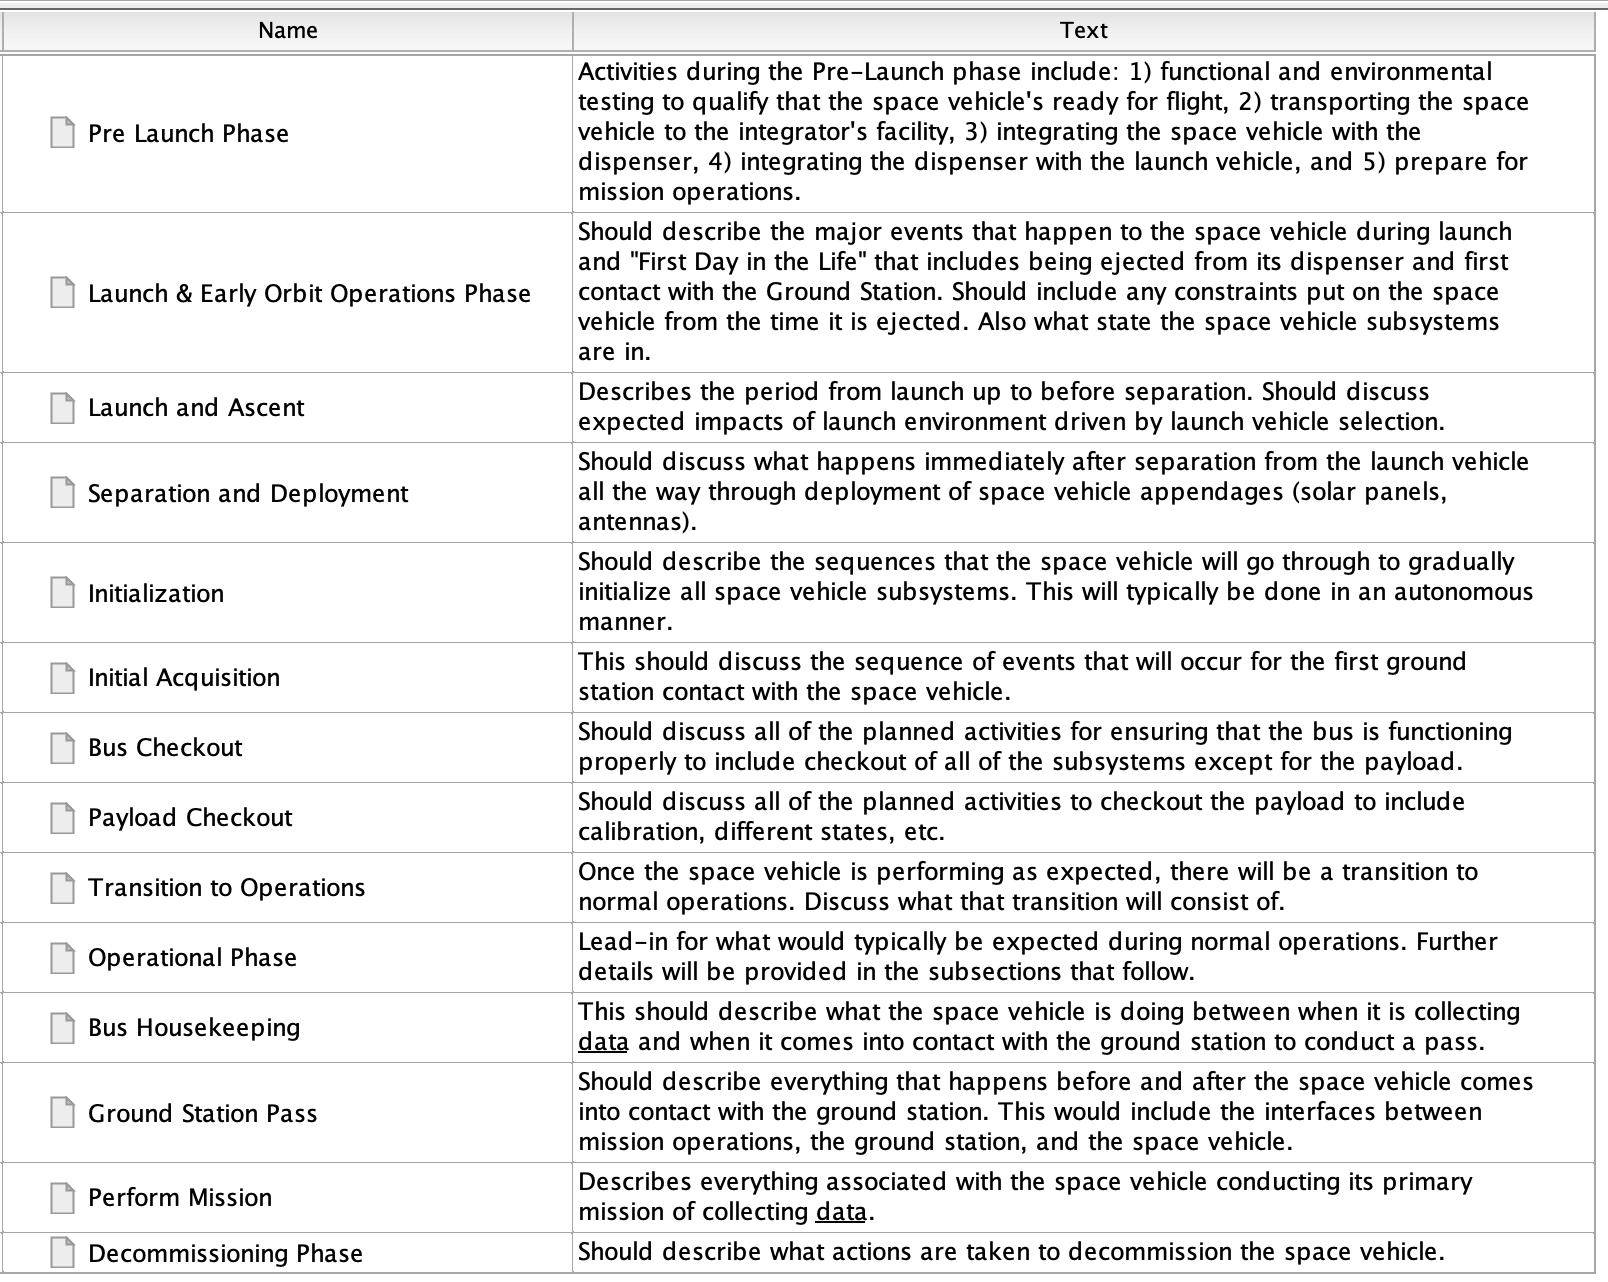
\includegraphics[width=\textwidth]{Thesis/Analysis_and_Results/Analysis and Results Figures/Mission Phase Descriptions.png}
    \caption{Mission Phase Descriptions}
    \label{fig:Mission Phase Descriptions}
\end{figure}

The Fault Management package, shown in Figure \ref{fig:Fault Management}, includes similar tables that will describe the various fault states in narrative form and in tables that shows each subsystem status.

\begin{figure}[H]
    \centering
    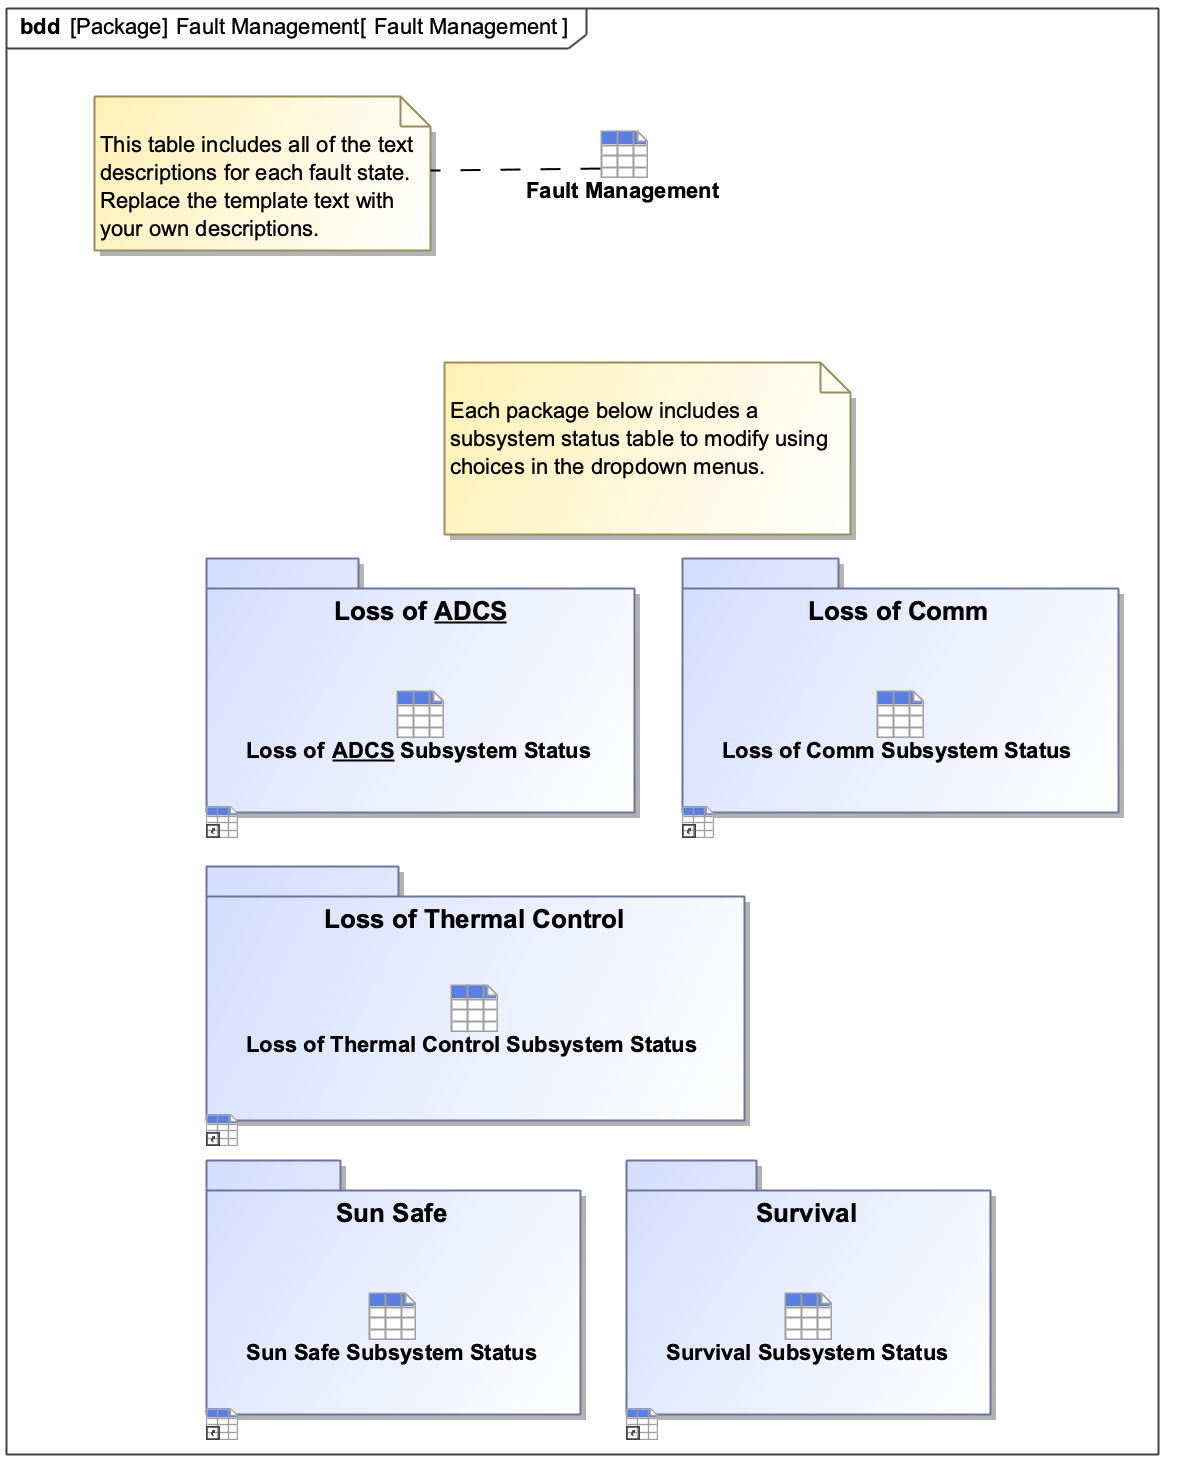
\includegraphics[width=4 in]{Thesis/Analysis_and_Results/Analysis and Results Figures/Fault Management.png}
    \caption{Fault Management}
    \label{fig:Fault Management}
\end{figure}

The CubeSat Activities package can hold any additional activities needed to describe the system. Activity diagrams for each critical mission phase have been created, although most only contain the starting and ending nodes. These vary substantially from mission to mission, so teams will need to populate these on their own. Finally, the Use Cases package includes a generic Use Case diagram that should be tailored.
